\documentclass[11pt,a4paper]{article}
\usepackage[utf8]{inputenc}
\usepackage[T1]{fontenc}
\usepackage{lmodern}
\usepackage[margin=2.2cm]{geometry}
\usepackage{amsmath,amssymb}
\usepackage{graphicx}
\usepackage{booktabs}
\usepackage{float}
\usepackage{icomma}
\usepackage[font=small,labelfont=bf]{caption}
\usepackage[hidelinks]{hyperref}

% No Polish babel in this TeX installation: Polish names set by hand
\renewcommand{\figurename}{Rysunek}
\renewcommand{\tablename}{Tabela}
\renewcommand{\refname}{Literatura}
\renewcommand{\contentsname}{Spis treści}
\setlength{\parindent}{0pt}
\setlength{\parskip}{0.6em}
\graphicspath{{figures/}}
\emergencystretch=1.5em

\title{Wielowarstwowa sieć neuronowa uczona propagacją wsteczną\\[0.3em]
  \large Sieci neuronowe, lista 3 (cz.~1 i 2): architektura, inicjalizacja i optymalizacja}
\author{Jeremiasz Lizak}
\date{29.10.2026}

\begin{document}
\maketitle

\section{Cel}
Celem było zaimplementowanie od podstaw (NumPy) wielowarstwowej sieci neuronowej z~aktywacją
ReLU i~kosztem entropii krzyżowej, uczonej algorytmem propagacji wstecznej, a~następnie
zbadanie jej zachowania na zbiorze Heart Disease.

W części~1 badano wpływ szerokości warstwy ukrytej, normalizacji danych i~liczby warstw
(wagi z~$\mathcal{N}(0, 0{,}01^2)$, współczynnik uczenia $\eta = 0{,}01$, pełny zbiór).
W~części~2 zaimplementowano optymalizator Adam, uczenie pełnym zbiorem, paczkami i~pojedynczymi
przykładami oraz wybór inicjalizacji wag, a~następnie porównano te warianty w~ustawieniach,
w~których problemy optymalizacji (płaskowyże, zanikające i~eksplodujące gradienty) są widoczne.

\section{Dane}
Wykorzystano ten sam zbiór i~podział co w~liście~2: połączone pliki \texttt{processed.*.data}
z~czterech ośrodków (918 pacjentów po usunięciu duplikatów, 13 cech). Zmienną \texttt{num}
zbinaryzowano ($\texttt{num} > 0 \to 1$), klasa pozytywna stanowi 55\%. Zera w~\texttt{trestbps}
i~\texttt{chol} potraktowano jako braki.

Dane podzielono warstwowo w~proporcji 60/20/20 (550/184/184). Imputacja (mediana lub dominanta),
kodowanie one-hot cech nominalnych i~standaryzacja są dopasowywane tylko na zbiorze treningowym.
Po przetworzeniu sieć dostaje $d = 27$ cech. W~wariancie bez normalizacji pominięto wyłącznie
standaryzację, więc np.\ cholesterol przyjmuje wartości do~603.

Krzywe uczenia pokazują stratę na zbiorze treningowym i~walidacyjnym. Metryki na zbiorze testowym
podano dla modelu po ostatniej epoce. Każdą konfigurację uczono z~trzema ziarnami losowania
(0,~1,~2). Wykresy pokazują średnią i~pasmo min--max, tabele średnią $\pm$ odchylenie standardowe.

\section{Implementacja}
Sieć zaimplementowano w~NumPy jako sekwencję warstw (klasa \texttt{Layer}), każda z~metodami
\texttt{forward} i~\texttt{backward}. Warstwy ukryte mają aktywację ReLU, warstwa wyjściowa ma
jeden neuron, na którego wyjście nakładana jest sigmoida. Kosztem jest średnia entropia krzyżowa.
W~\texttt{forward} warstwa zapamiętuje swoje wejście i~wartość przed aktywacją, w~\texttt{backward}
zapisuje gradienty po wagach i~biasie i~zwraca gradient po wejściu do poprzedniej warstwy.

Poprawność gradientów sprawdzono numerycznie (różnica centralna, $\varepsilon = 10^{-5}$) na sieci
$4 \to 6 \to 5 \to 4 \to 1$ dla wszystkich wag i~biasów. Maksymalny błąd względny wyniósł
$3\cdot10^{-9}$.

W~części~2 dodano:
\begin{itemize}
  \item wybór inicjalizacji wag: $\mathcal{N}(0, \sigma^2)$ ze stałym $\sigma$ albo He
    ($\sigma = \sqrt{2/d_{in}}$ osobno dla każdej warstwy); biasy zawsze startują od zera,
  \item uczenie paczkami o~rozmiarze $B$ z~tasowaniem zbioru w~każdej epoce: $B = 550$ (pełny zbiór),
    $B = 32$ (paczki), $B = 1$ (pojedyncze przykłady),
  \item optymalizatory jako osobne klasy: zwykły spadek gradientu i~Adam
    ($\beta_1 = 0{,}9$, $\beta_2 = 0{,}999$, $\epsilon = 10^{-8}$, $\alpha = 0{,}001$).
\end{itemize}

\section{Część 1: architektura i normalizacja}
Ustawienia z~listy: pełny zbiór, $\eta = 0{,}01$, wagi z~$\mathcal{N}(0, 0{,}01^2)$, 20\,000 epok.
Wyniki zebrano w~tabeli~\ref{tab:p1}.

\begin{table}[H]
\centering
\begin{tabular}{llccc}
\toprule
badanie & konfiguracja & strata tren. & strata walid. & accuracy test \\
\midrule
szerokość & 1 ukryta, 3 neurony & 0,348 $\pm$ 0,006 & 0,441 $\pm$ 0,010 & 0,835 $\pm$ 0,003 \\
          & 1 ukryta, 27 neuronów ($= d$) & 0,294 $\pm$ 0,011 & 0,450 $\pm$ 0,007 & 0,846 $\pm$ 0,007 \\
          & 1 ukryta, 270 neuronów & 0,239 $\pm$ 0,005 & 0,482 $\pm$ 0,004 & 0,848 $\pm$ 0,004 \\
\midrule
normalizacja & znormalizowane & 0,294 $\pm$ 0,011 & 0,450 $\pm$ 0,007 & 0,846 $\pm$ 0,007 \\
             & nieznormalizowane & 0,605 $\pm$ 0,063 & 0,686 $\pm$ 0,067 & 0,652 $\pm$ 0,077 \\
\midrule
głębokość & 1 ukryta $\times$ 27 & 0,294 $\pm$ 0,011 & 0,450 $\pm$ 0,007 & 0,846 $\pm$ 0,007 \\
          & 2 ukryte $\times$ 27 & 0,293 $\pm$ 0,032 & 0,451 $\pm$ 0,017 & 0,835 $\pm$ 0,005 \\
          & 3 ukryte $\times$ 27 & 0,688 $\pm$ 0,000 & 0,687 $\pm$ 0,000 & 0,554 $\pm$ 0,000 \\
          & 4 ukryte $\times$ 27 & 0,688 $\pm$ 0,000 & 0,687 $\pm$ 0,000 & 0,554 $\pm$ 0,000 \\
\bottomrule
\end{tabular}
\caption{Część~1, wyniki po 20\,000 epokach.}
\label{tab:p1}
\end{table}

\subsection{Szerokość warstwy ukrytej}
\begin{figure}[H]
\centering
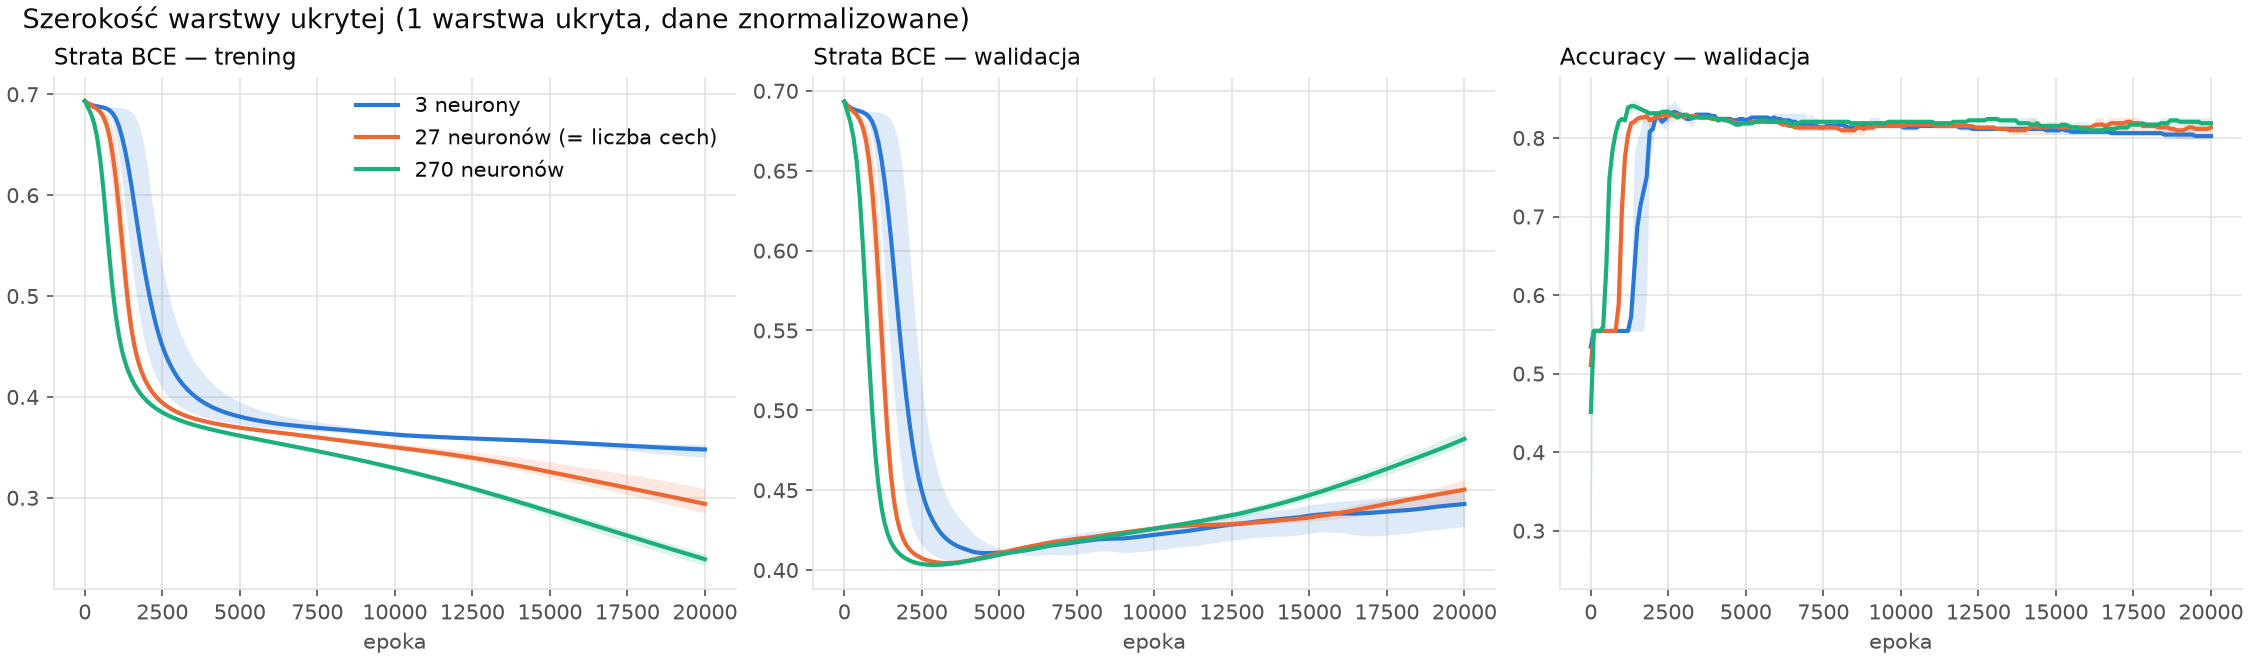
\includegraphics[width=\textwidth]{hidden_width.png}
\caption{Krzywe uczenia dla różnej liczby neuronów w~jedynej warstwie ukrytej.}
\label{fig:width}
\end{figure}

Większa warstwa ukryta lepiej dopasowuje się do zbioru treningowego (strata 0,348 dla 3 neuronów,
0,239 dla 270), ale na zbiorze walidacyjnym i~testowym różnice mieszczą się w~granicach szumu
(184 próbki). Wszystkie warianty osiągają najniższą stratę walidacyjną około 3000.\ epoki,
a~później ta strata rośnie, czyli sieć zaczyna się przeuczać. Efekt jest najsilniejszy dla
270 neuronów (rys.~\ref{fig:width}). Już 3 neurony wystarczają, żeby dorównać regresji
logistycznej z~listy~2 (accuracy 0,837), co pasuje do tego, że ten zbiór jest w~dużej mierze
liniowo separowalny.

\subsection{Normalizacja danych}
\begin{figure}[H]
\centering
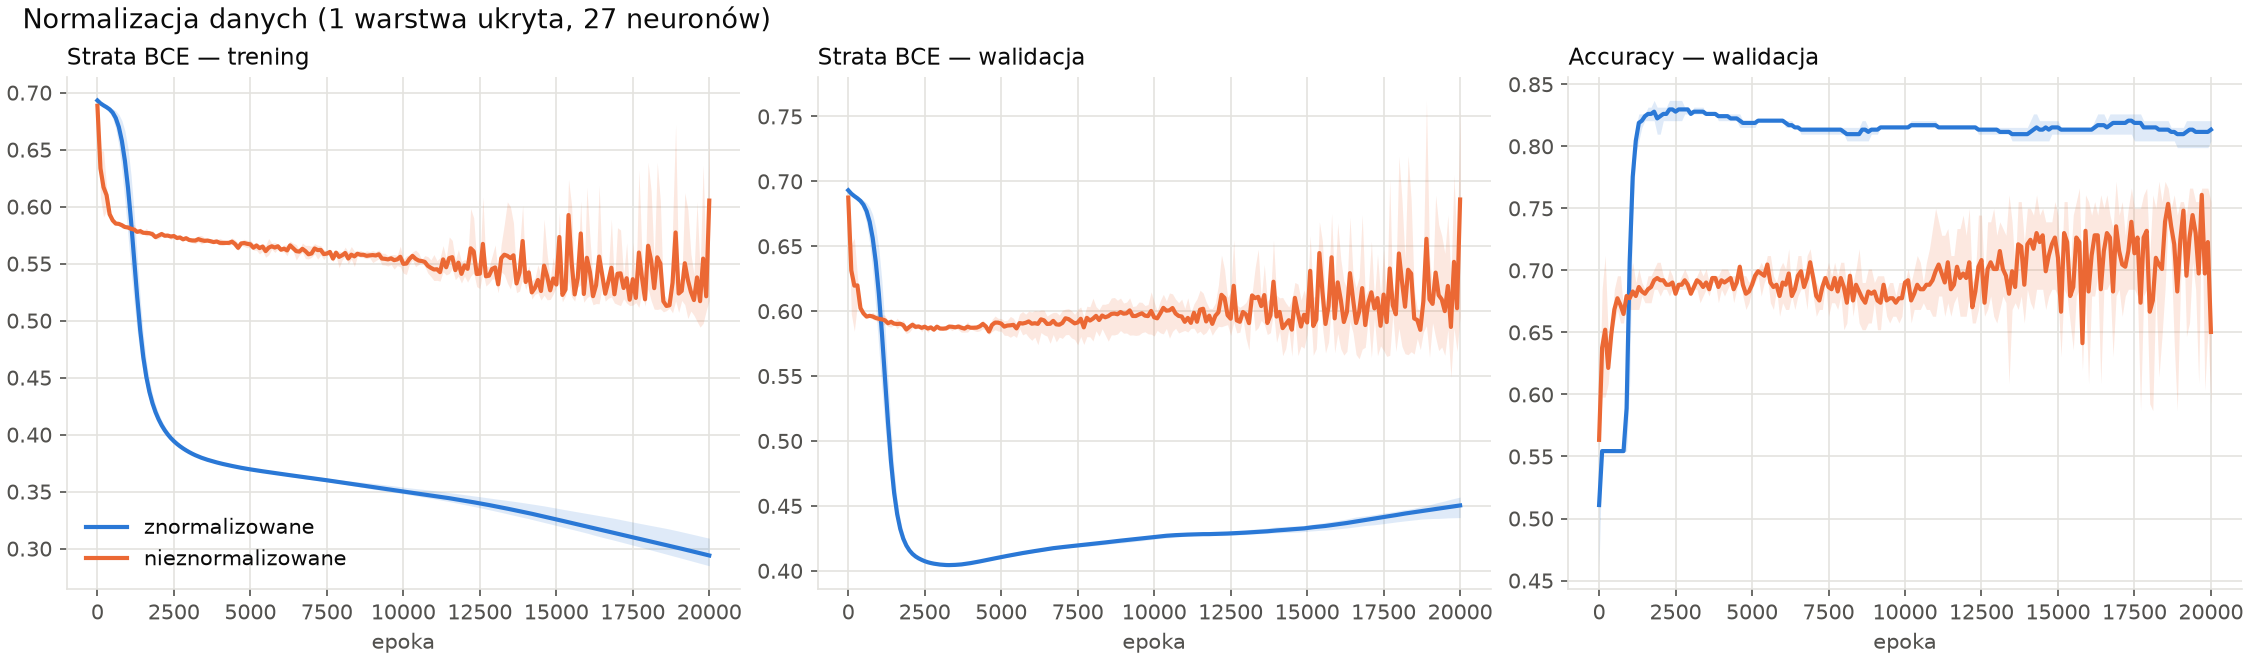
\includegraphics[width=\textwidth]{normalization.png}
\caption{Krzywe uczenia dla danych znormalizowanych i~nieznormalizowanych (1 warstwa ukryta, 27 neuronów).}
\label{fig:norm}
\end{figure}

Bez standaryzacji cechy mają skale od 0--1 (cechy binarne) do kilkuset (\texttt{chol}).
Strata spada szybko tylko
w~pierwszych epokach, potem oscyluje (rys.~\ref{fig:norm}), a~accuracy testowe wynosi 0,652
zamiast 0,846. Wyniki zależą też mocno od ziarna (odchylenie 0,077).

\subsection{Liczba warstw}
\begin{figure}[H]
\centering
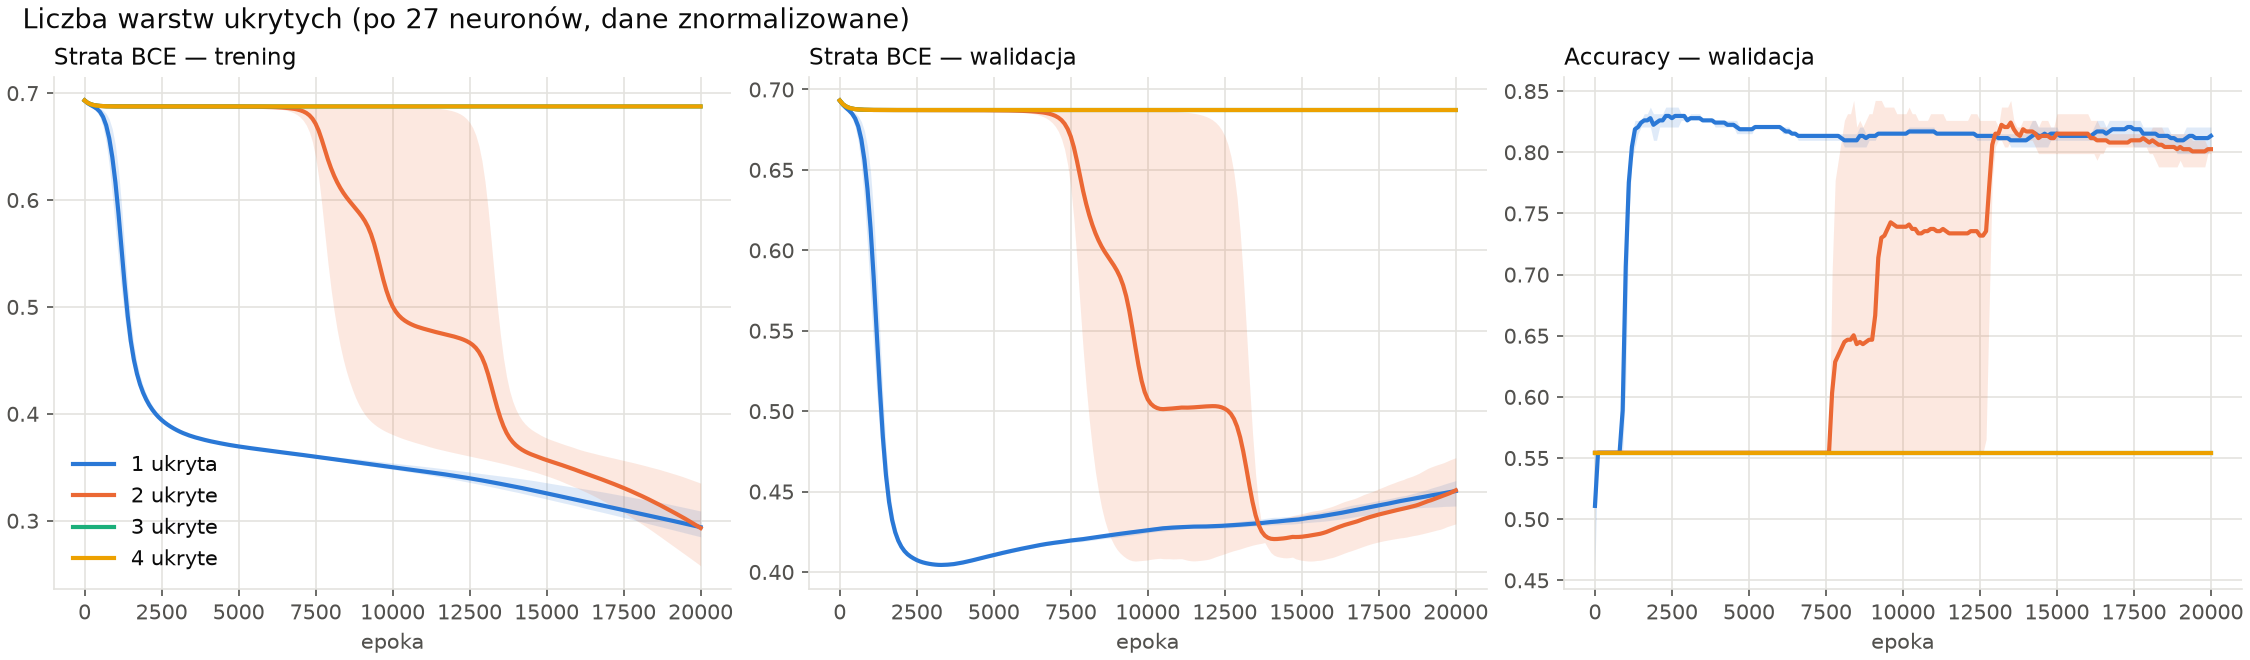
\includegraphics[width=\textwidth]{depth.png}
\caption{Krzywe uczenia dla różnej liczby warstw ukrytych (po 27 neuronów). Linie dla 3 i~4
warstw pokrywają się.}
\label{fig:depth}
\end{figure}

Sieć z~jedną warstwą ukrytą uczy się od razu, z~dwiema stoi na płaskowyżu przez około 7500 epok,
zanim strata zacznie spadać (rys.~\ref{fig:depth}). Sieci z~3 i~4 warstwami w~ciągu 20\,000 epok
w~ogóle nie wychodzą z~płaskowyżu. Uczy się w~nich praktycznie tylko bias ostatniej warstwy,
więc model zwraca stałe prawdopodobieństwo równe udziałowi klasy pozytywnej (strata 0,688,
accuracy 0,554).

\section{Część 2: optymalizacja}
Głębokość sieci i~liczbę epok w~każdym badaniu dobrano tak, żeby badany problem był widoczny.
We~wszystkich badaniach warstwy ukryte mają po 27 neuronów, a~zwykły spadek gradientu używa
$\eta = 0{,}01$. Wyniki zebrano w~tabeli~\ref{tab:p2}.

\begin{table}[H]
\centering
\small
\begin{tabular}{llcccccc}
\toprule
badanie & konfiguracja & strata tren. & min.\ str.\ walid. & accuracy & F1 & ROC AUC \\
\midrule
tryb       & pełny zbiór (550) & 0,688 & 0,687 & 0,554 & 0,713 & 0,744 \\
(2 ukryte) & paczki (32)       & 0,325 & 0,405 & 0,842 & 0,863 & 0,921 \\
           & pojedyncze (1)    & 0,000 & 0,396 & 0,804 & 0,825 & 0,873 \\
\midrule
inicjalizacja & $\mathcal{N}(0, 0{,}01^2)$ & 0,688 & 0,687 & 0,554 & 0,713 & 0,714 \\
(4 ukryte)    & $\mathcal{N}(0, 1)$        & 0,041 & 2,319 & 0,716 & 0,748 & 0,773 \\
              & He                         & 0,164 & 0,433 & 0,813 & 0,835 & 0,901 \\
              & $\mathcal{N}(0, 10^2)$     & 0,688 & 0,687 & 0,554 & 0,713 & 0,500 \\
\midrule
optymalizator & gradient, $\mathcal{N}(0, 0{,}01^2)$ & 0,688 & 0,687 & 0,554 & 0,713 & 0,548 \\
(6 ukrytych)  & Adam, $\mathcal{N}(0, 0{,}01^2)$     & 0,134 & 0,410 & 0,832 & 0,848 & 0,891 \\
              & gradient, He                         & 0,048 & 0,439 & 0,806 & 0,830 & 0,876 \\
              & Adam, He                             & 0,021 & 0,451 & 0,788 & 0,809 & 0,874 \\
\bottomrule
\end{tabular}
\caption{Część~2, średnie z~trzech ziaren. Strata treningowa i~metryki testowe po ostatniej
epoce, strata walidacyjna minimalna w~trakcie uczenia. Accuracy, F1 i~ROC AUC na zbiorze
testowym. F1 = 0,713 przy accuracy 0,554 oznacza model, który zawsze przewiduje klasę 1.}
\label{tab:p2}
\end{table}

\subsection{Pełny zbiór, paczki i pojedyncze przykłady}
Użyto ustawienia z~części~1, w~którym pełny zbiór utknął na długim płaskowyżu: 2 warstwy ukryte,
wagi z~$\mathcal{N}(0, 0{,}01^2)$, zwykły spadek gradientu. Każdy wariant dostał 1000 epok.

\begin{figure}[H]
\centering
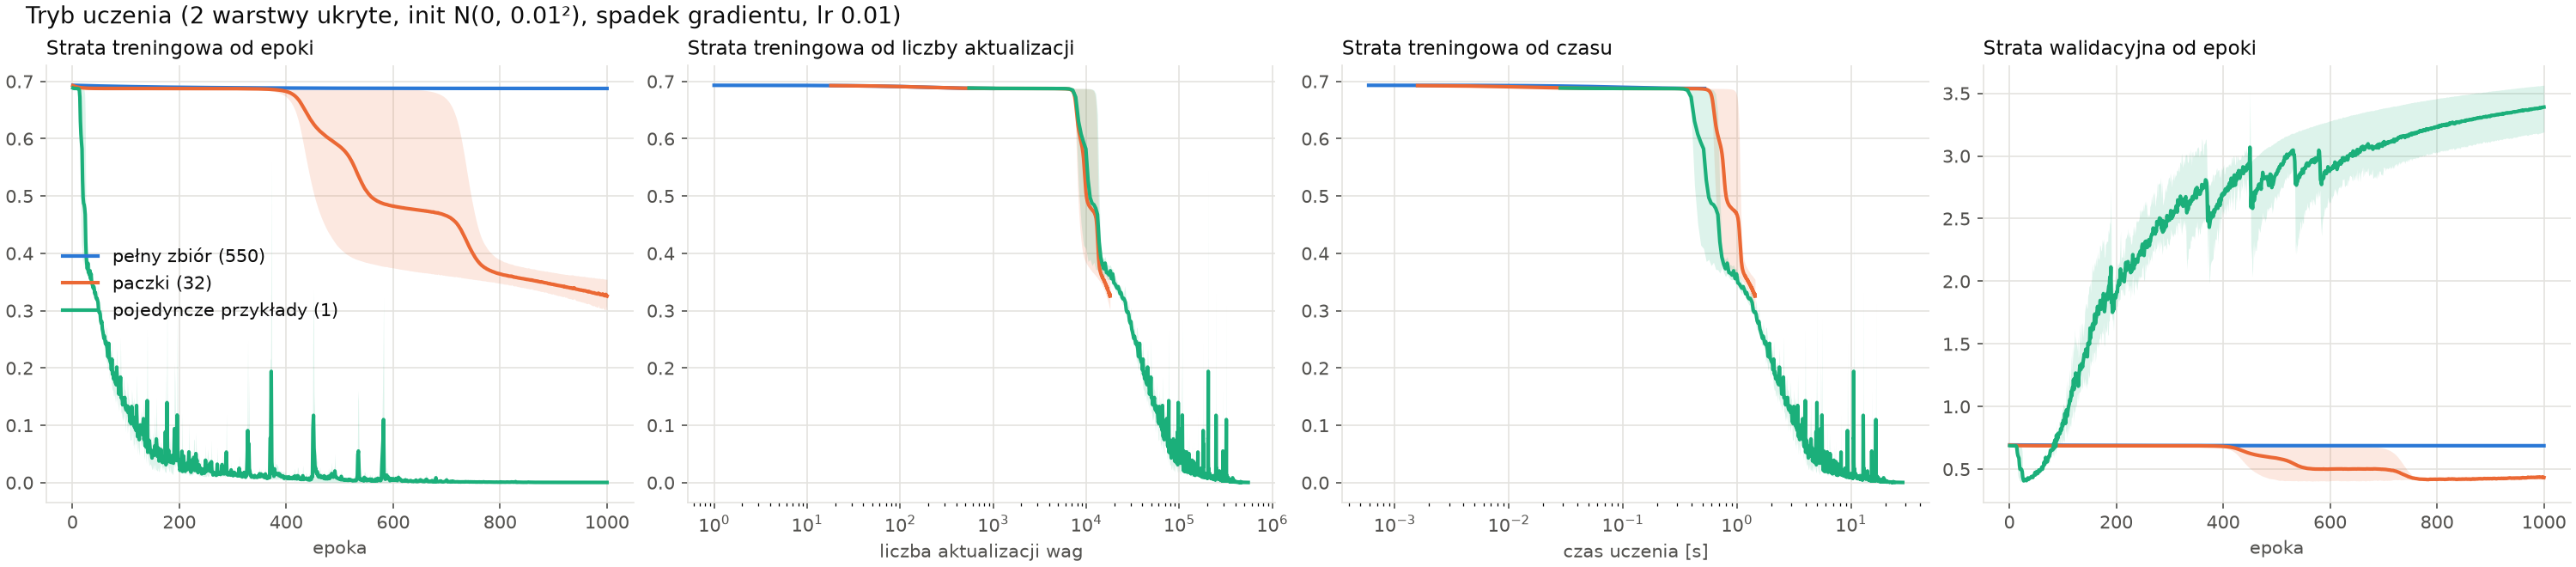
\includegraphics[width=\textwidth]{p2_batch.png}
\caption{Tryby uczenia. Ta sama strata treningowa na osi epok, liczby aktualizacji wag i~czasu
uczenia (dwie ostatnie osie logarytmiczne) oraz strata walidacyjna.}
\label{fig:batch}
\end{figure}

Na osi epok różnica jest ogromna (rys.~\ref{fig:batch}). Pełny zbiór przez 1000 epok nie opuszcza
płaskowyżu, paczki opuszczają go po 400--750 epokach, a~pojedyncze przykłady po około 15.
Na wykresie od liczby aktualizacji wag we wszystkich trybach wyjście
z~płaskowyżu następuje po podobnej liczbie kroków, około $10^4$. Tyle samo potrzebował pełny
zbiór w~części~1 (7500--13\,000 epok). Mniejsze paczki wykonują więcej kroków na epokę, a~sam płaskowyż
liczony w~krokach był we wszystkich trybach podobny.

Na osi czasu paczki i~pojedyncze przykłady opuszczają płaskowyż w~podobnym czasie (około 1~s).
Pojedyncze przykłady prowadzą jednak do silnego przeuczenia. Strata treningowa spada do zera,
walidacyjna rośnie do 3,4 (minimum 0,396 po kilkunastu epokach), a~krzywa jest bardzo zaszumiona.
Najlepszy wynik testowy dały paczki (accuracy 0,842, F1 0,863), przy czasie 1,4~s wobec 28~s dla
pojedynczych przykładów.

\subsection{Inicjalizacja wag}
Sieć z~4 warstwami ukrytymi uczono paczkami po 32 przez 200 epok. Oprócz trzech wariantów z~listy
dodano $\mathcal{N}(0, 0{,}01^2)$ z~części~1. Przed uczeniem zmierzono normę gradientu w~każdej warstwie.

\begin{figure}[H]
\centering
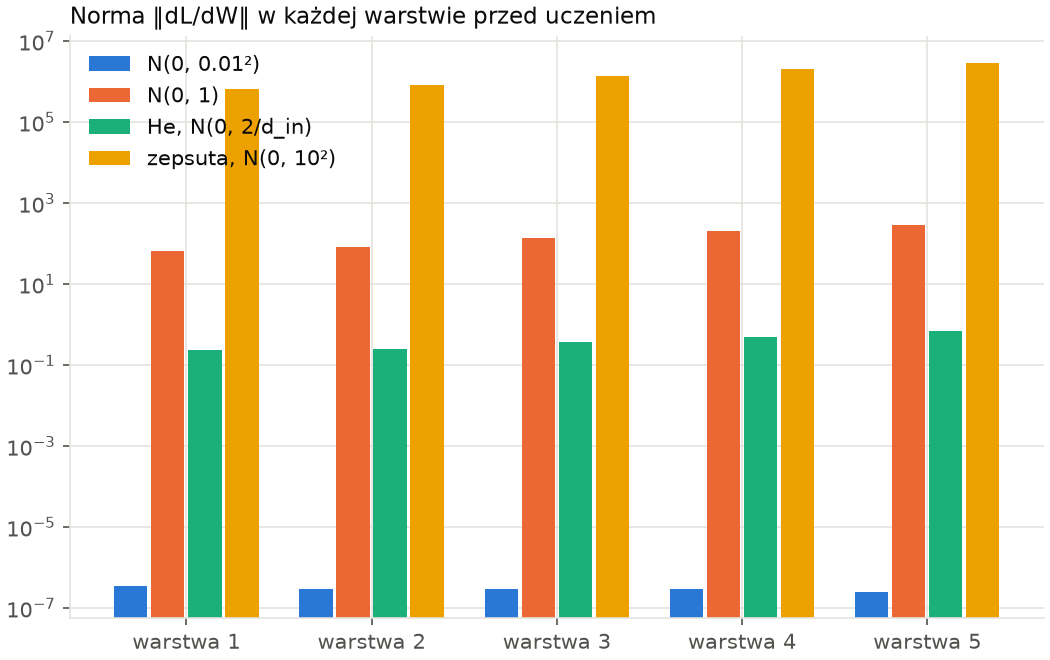
\includegraphics[width=0.62\textwidth]{p2_init_grad_norms.png}
\caption{Norma $\lVert \partial L/\partial W \rVert$ w~każdej warstwie przed rozpoczęciem uczenia
(skala logarytmiczna, warstwa~5 to warstwa wyjściowa).}
\label{fig:gradnorms}
\end{figure}

\begin{figure}[H]
\centering
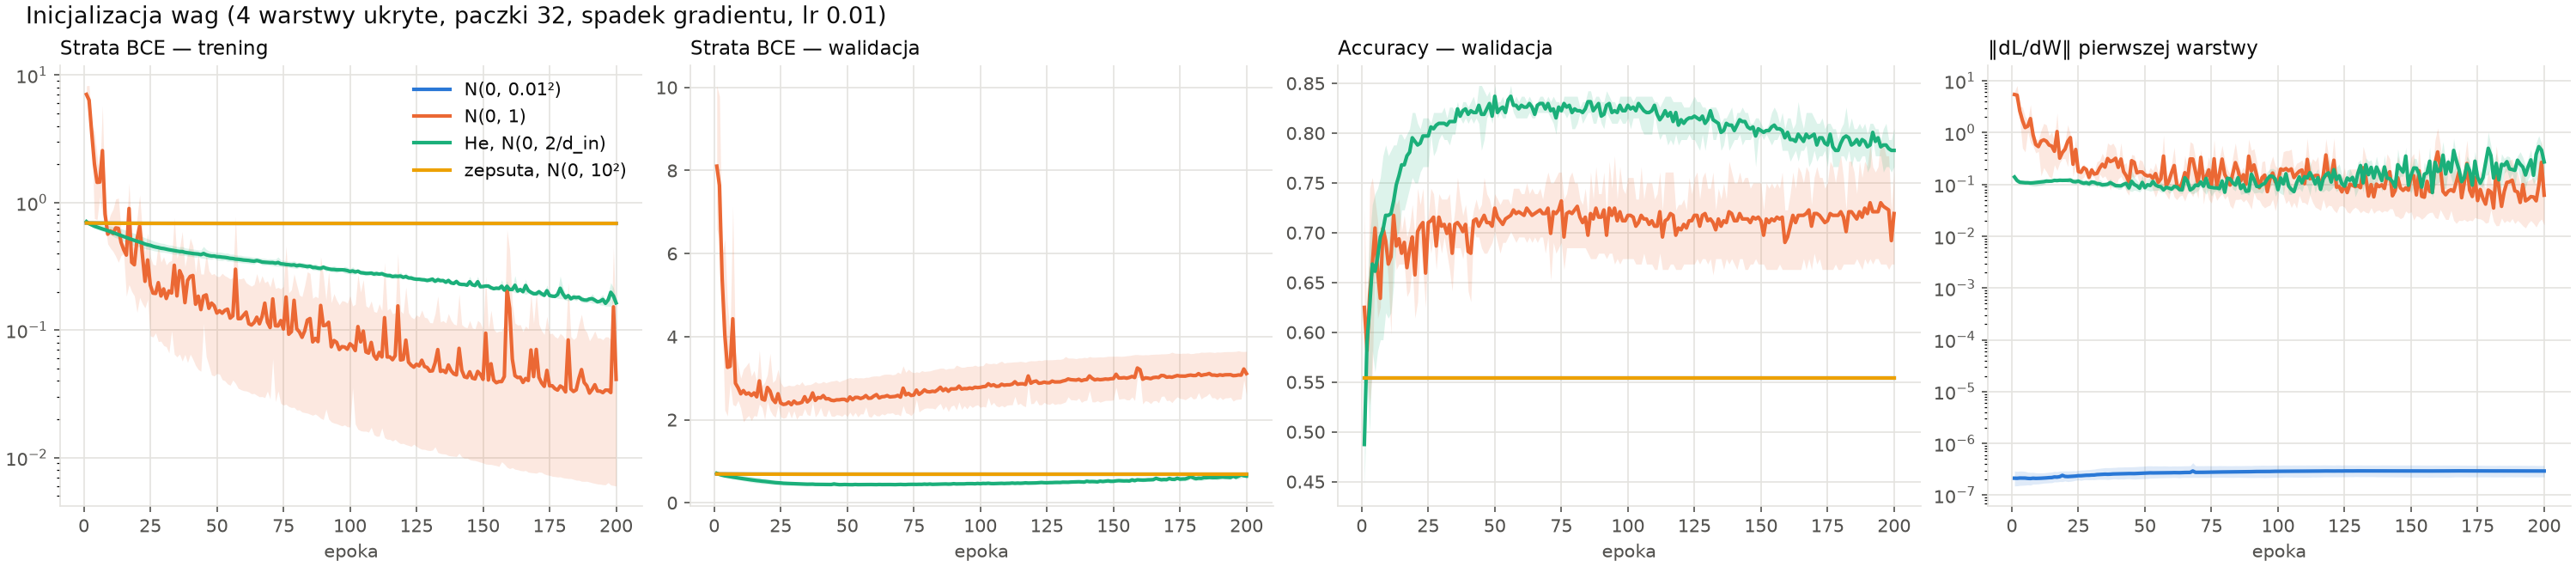
\includegraphics[width=\textwidth]{p2_init.png}
\caption{Krzywe uczenia dla różnych inicjalizacji (strata treningowa i~norma gradientu w~skali
logarytmicznej). Dla $\mathcal{N}(0, 10^2)$ norma gradientu wynosi dokładnie 0, więc nie ma jej na wykresie.}
\label{fig:init}
\end{figure}

Rysunek~\ref{fig:gradnorms} pokazuje skalę gradientów na starcie. Dla $\sigma = 0{,}01$ norma
gradientu w~pierwszej warstwie wynosi około $3\cdot10^{-7}$, dla He 0,24, dla $\sigma = 1$
około 67, a~dla $\sigma = 10$ około $7\cdot10^{5}$. Te cztery inicjalizacje prowadzą do czterech
różnych przebiegów (rys.~\ref{fig:init}):
\begin{itemize}
  \item \textbf{$\mathcal{N}(0, 0{,}01^2)$}: gradienty zanikają, sieć przez 200 epok stoi na
    płaskowyżu i~zwraca stałą (accuracy 0,554).
  \item \textbf{$\mathcal{N}(0, 1)$}: początkowa strata wynosi około 7. Uczenie przebiega skokami. Sieć szybko zapamiętuje zbiór treningowy (strata 0,041),
    ale strata walidacyjna nigdy nie spada poniżej 2,3, a~accuracy testowe to tylko 0,716.
  \item \textbf{He}: norma gradientu jest podobna we wszystkich warstwach i~bliska 1, strata spada
    od pierwszej epoki. To jedyny wariant z~dobrym wynikiem (accuracy 0,813, AUC 0,901).
  \item \textbf{$\mathcal{N}(0, 10^2)$} (zepsuta): gradienty rzędu $10^6$ sprawiają, że po
    czterech krokach wagi osiągają wartości rzędu $10^{75}$--$10^{108}$, a~wyjście sieci skacze
    między 0 a~1. Po 5--6 krokach w~warstwach 2--4 nie ma już żadnego neuronu z~$z > 0$ dla
    jakiejkolwiek próbki. Już pod koniec pierwszej epoki
    gradient wszystkich warstw ukrytych jest dokładnie zerowy, uczy się tylko bias wyjścia, a~sieć
    zwraca stałą (AUC 0,5).
\end{itemize}

\subsection{Spadek gradientu a Adam}
Użyto głębszej sieci, z~6 warstwami ukrytymi (paczki 32, 200 epok). Porównano oba optymalizatory
przy małej inicjalizacji, gdzie gradient praktycznie zanika, i~przy inicjalizacji He.

\begin{figure}[H]
\centering
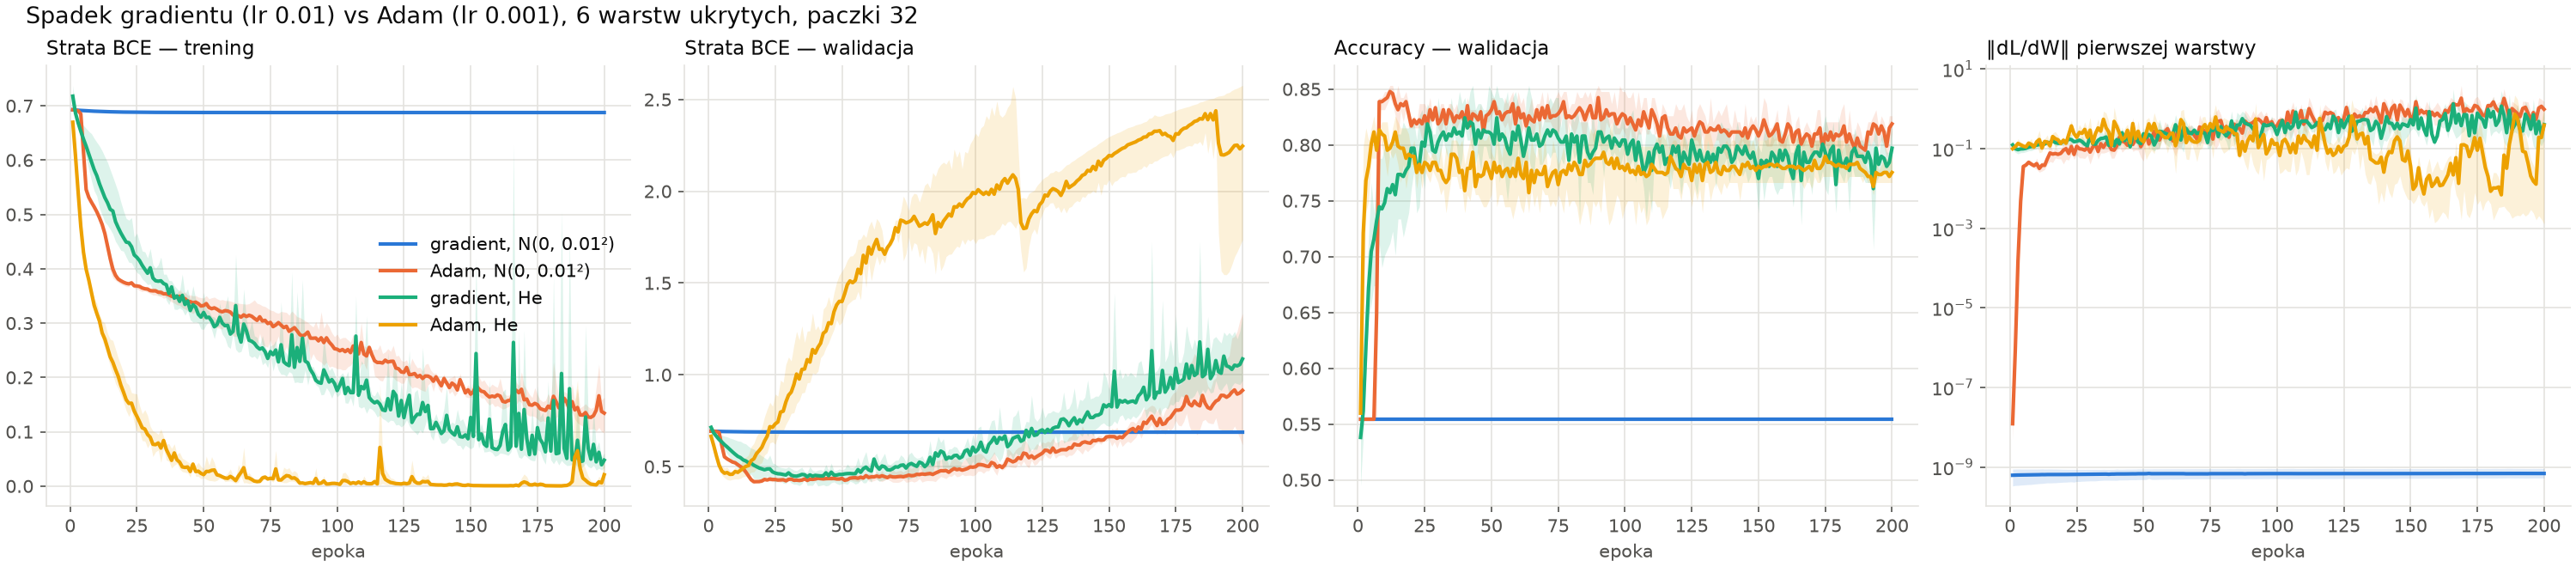
\includegraphics[width=\textwidth]{p2_adam.png}
\caption{Zwykły spadek gradientu ($\eta = 0{,}01$) i~Adam ($\alpha = 0{,}001$) dla dwóch inicjalizacji.}
\label{fig:adam}
\end{figure}

Przy $\mathcal{N}(0, 0{,}01^2)$ norma gradientu pierwszej warstwy wynosi około $10^{-9}$
i~zwykły spadek gradientu w~ciągu 200 epok nie zmienia straty (rys.~\ref{fig:adam}). Adam wychodzi
z~płaskowyżu po kilku epokach, a~norma gradientu rośnie o~8 rzędów wielkości. Ten wariant osiągnął najlepszy
wynik testowy w~tym badaniu (accuracy 0,832, F1 0,848).

Przy inicjalizacji He oba optymalizatory uczą się od początku, a~Adam szybciej zmniejsza stratę
treningową (0,021 wobec 0,048). Szybciej też zaczyna się przeuczać: strata walidacyjna osiąga
minimum po około 10 epokach i~rośnie do 2,25 na końcu uczenia. Krok Adama jest około 1,8 raza droższy (1,16~s wobec 0,64~s na 200 epok).

\subsection{Warunek stopu}
Do każdego przebiegu policzono, w~której epoce zatrzymałoby uczenie kryterium z~listy~2:
spadek straty treningowej między epokami mniejszy niż $\mathrm{tol} = 10^{-6}$.

\begin{table}[H]
\centering
\small
\begin{tabular}{lcc}
\toprule
konfiguracja & zatrzymanie przy tol $= 10^{-6}$ & faktyczne wyjście z~płaskowyżu \\
\midrule
pełny zbiór, 2 ukryte          & epoka 669 & po 7500--13\,000 epokach (cz.~1) \\
paczki 32, 2 ukryte            & epoka 25  & epoka 400--750 \\
pojedyncze przykłady, 2 ukryte & epoka 5   & epoka $\approx$ 15 \\
gradient, 6 ukrytych, $\mathcal{N}(0, 0{,}01^2)$ & epoka 24 & nie nastąpiło \\
Adam, 6 ukrytych, $\mathcal{N}(0, 0{,}01^2)$     & epoka 26 & epoka $\approx$ 5 \\
\bottomrule
\end{tabular}
\caption{Epoka, w~której zatrzymałby uczenie warunek stopu oparty na spadku straty (średnia z~trzech ziaren).}
\label{tab:tol}
\end{table}

W~każdym przypadku z~płaskowyżem warunek zatrzymałby uczenie, zanim sieć zaczęła się uczyć
(tabela~\ref{tab:tol}). Przy Adamie zadziałało dopiero po wyjściu z~płaskowyżu. Dlatego
wszystkie badania w~tej części mają stałą liczbę epok.

\section{Wnioski}
\begin{itemize}
  \item Gradienty z~propagacji wstecznej zgadzają się z~numerycznymi z~dokładnością $10^{-9}$.
  \item Już sieć z~jedną warstwą ukrytą dorównuje regresji logistycznej z~listy~2. Szersza warstwa
    ukryta poprawia tylko dopasowanie do zbioru treningowego. Bez normalizacji danych accuracy
    spada z~0,846 do 0,652.
  \item Przy wagach z~$\mathcal{N}(0, 0{,}01^2)$ sieć z~2 warstwami ukrytymi zaczyna się uczyć
    dopiero po około 7500 epokach, a~z~3 i~więcej nie uczy się wcale. Przy $\mathcal{N}(0, 10^2)$
    sieć po kilku krokach przestaje się uczyć. W~obu przypadkach model zwraca stałą.
  \item Z~badanych inicjalizacji tylko He pozwoliła głębokiej sieci uczyć się zwykłym spadkiem
    gradientu od pierwszej epoki.
  \item Adam wyszedł z~płaskowyżu, na którym zwykły spadek gradientu stał. Przy inicjalizacji He
    szybciej zmniejszał stratę, ale też szybciej się przeuczał.
  \item Mniejsze paczki skróciły płaskowyż liczony w~epokach, liczony w~krokach był podobny.
    Paczki 32 dały najlepszy wynik testowy przy krótkim czasie uczenia.
  \item Warunek stopu oparty na spadku straty treningowej zatrzymałby uczenie na płaskowyżu
    we wszystkich przypadkach, w~których płaskowyż wystąpił.
\end{itemize}

\end{document}
